

\section{Policy Parameterization}
\label{section:optimization}

% While our gradient estimation framework offers a sample-efficient alternative for learning from the environment, there is another practical issue that degrades the performance of learning algorithms for queuing control: stability. It has been observed that standard reinforcement learning algorithms, which are usually initialized at a random policy, can fail to stabilize queuing networks. As a result, researchers have proposed modifications to ensure stability, including behavior cloning of a stabilizing policy~\cite{dai2022queueing}, switching to a stabilizing policy if the queue-lengths exceed a specified level~\cite{liu2022rl}, or shaping the costs to be stability-aware. 
While our gradient estimation framework 
offers a sample-efficient alternative for 
learning from the environment, there is another practical 
issue that degrades the performance of learning algorithms for 
queuing network control: instability. Standard model-free RL algorithms are based on the `tabula rasa' principle, which aims to search over a general and unstructured policy class in order to find an optimal policy. However, it has been observed that this approach may be unsuitable for queuing network control. Due to the lack of structure, the policies visited by the algorithm often fail to stabilize the network,
which prevents the algorithm from learning and improving.
As a result, researchers have proposed structural modifications to ensure stability, 
including behavior cloning of a stabilizing policy to find a good initialization~\cite{dai2022queueing}, 
switching to a stabilizing policy 
if the queue lengths exceed some finite thresholds~\cite{liu2022rl}, 
or modifying the costs to be stability-aware~\cite{pavse2024learning}. 
% \hntodo{CITE}

We investigate the source of instability in various queuing scheduling problems and find a possible explanation. 
We note that many policies obtained by model-free RL algorithms are not {\bf work-conserving} and often allocate servers to empty queues. A scheduling policy is work-conserving if it always keeps the server(s) busy when there are compatible jobs waiting to be served.
%Work-conservation is a well-studied propertyin the queuing literature, and is usually a pre-condition for a policy to induce stability in the queuing network. 
Standard policies such as the $c\mu$-rule, MaxPressure, and MaxWeight are all work-conserving, which partly explains their success in stabilizing complex networks. We treat work conservation as an `inductive bias'
% \hntodo{Most queueing and applied probability people will have no idea what this word means. Spend 2-3 sentences providing background on how this is the key modeling lever in ML and has been responsible for most practical success.} 
and consider a simple modification to the policy architecture that guarantees this property without sacrificing the flexibility of the policy class. 

The de-facto approach for parameterizing policies in deep reinforcement learning is to consider a function $\nu_{\theta}(x)$,
which belongs to a general function family, such as neural networks, and outputs real-valued scores.
These scores are then fed into a $\softmax$ layer, which converts the scores to probabilities over actions.
Naively, the number of possible routing actions can grow exponentially in the number of queues and servers.
Nonetheless, one can efficiently sample from the action space by having the output of
$\nu_{\theta}(x) \in \R^{m\times n}$ be a matrix where row $i$, denote as $\nu_{\theta}(x)_{i}$, contains the scores for matching server $i$ to different queues. Then by applying the $\softmax$ for row $i$, i.e., $\softmax(\nu_{\theta}(x)_{i})$, we obtain the probability that server $i$ is assigned to each queue. We then sample the assignment independently for each server to obtain an action in $\mathcal{U}$.
For the purpose of computing the $\pathwise$ estimator, $\softmax(\nu_{\theta}(x)_{i})$ also gives a valid fractional routing in $\overline{\mathcal{U}}$. We let $\softmax(\nu_{\theta}(x))\in \overline{\mathcal{U}}$ denote the matrix formed by applying the softmax to each row in $\nu_{\theta}(x)$.



Under this `vanilla' softmax policy, the probability $\pi_{\theta}(x)_{ij}$ that server $i$ is routed to queue $j$ 
(or alternatively, the fractional capacity server $i$ allocated to $j$) is given by
\begin{equation}
\label{eq:vanilla_softmax}
\pi_{\theta}(x)_{ij} = \softmax(\nu_{\theta}(x))_{ij} = \frac{e^{\nu_{\theta}(x)_{ij}}}{\sum_{j=1}^{n} e^{\nu_{\theta}(x)_{ij}}}. \hspace{-3em}
\tag{Vanilla Softmax}
\end{equation}
Many of the policies mentioned earlier can be defined in this way, such as the soft MaxWeight policy, $\nu_{\theta}(x)_{i} = \{ \theta_{j}x_{j}\mu_{ij}\}_{j=1}^{n}$. This parameterization is highly flexible
and $\nu_{\theta}(x)$
can be the output of a neural network. However, for a general $\nu_{\theta}(x)$,
there is no guarantee that $\pi(\theta)(x)_{i,j} = 0$ if $x_{j} = 0$. This means that such policies
may waste service capacity by allocating capacity to empty queues even when there are non-empty queues that 
server $i$ could work on.

We propose a simple fix, which reshapes the actions produced by the policy.
We refer to this as the {\bf work-conserving $\softmax$},
% \[
% \bar{\pi}_{\theta}(x)_{i,j} \proto \pi_{\theta}(x)_{i,j}1{x_{j} > 0} \wedge \epsilon \propto e^{\nu_{\theta}(x)_{i,j}}1{x_{j} > 0} \wedge \epsilon
% \]
\begin{equation}
\label{eq:work-conserving}
    \pi_{\theta}^{\mathsf{WC}}(x)_{ij} = \mathsf{softmaxWC}(\nu_{\theta}(x))_{ij} \equiv \frac{e^{\nu_{\theta}(x)_{ij}}1\{x_{j} > 0\}\wedge \epsilon}
{\sum_{l=1}^{n} e^{\nu_{\theta}(x)_{il}}1\{x_{l} > 0\}\wedge \epsilon},
\hspace{-3em}
\tag{WC-Softmax}
\end{equation}
where $\wedge$ is the minimum and $\epsilon$ is a small number to prevent
division by zero when the queue lengths are all zero.

This parameterization is fully compatible with deep reinforcement learning approaches.
$\nu_{\theta}(x)$ can be a neural network and critically, the work-conserving $\softmax$
preserves the differentiability of $\pi^{\mathsf{WC}}_{\theta}(x)$ with respect to $\theta$.
As a result, $\reinforce$ and $\pathwise$ estimators can both be computed under this parameterization, since $\nabla_{\theta} \log \pi_{\theta}^{\mathsf{WC}}(x)$ and $\nabla_{\theta} \pi_{\theta}^{\mathsf{WC}}(x)$
both exist.

This simple modification delivers substantial improvements in performance. Figure~\ref{fig:work-conserving} compares the average holding cost across policy iterations for PPO without any modifications, PPO initialized with a policy trained to imitate MaxWeight, and PPO with the work-conserving $\softmax$. Despite its empirical success in many other reinforcement learning problems, PPO without any modifications fails to stabilize the network and incurs an exceedingly high cost. It performs much better under an initial behavioral cloning step, which achieves stability but still underperforms the $c\mu$-rule. On the other hand, with the work-conserving $\softmax$, even the randomly initialized policy stabilizes the network and outperforms the $c\mu$-rule over the course of training. This illustrates that an appropriate choice of policy architecture, motivated by queuing theory, is decisive in enabling learning-based approaches to succeed. As a result, for all of the policy optimization experiments in sections~\ref{section:learn_cmu},~\ref{section:admission}, and~\ref{section:results}, we equip the policy parameterization with the work-conserving $\softmax$.

\begin{figure}[t]
\centering
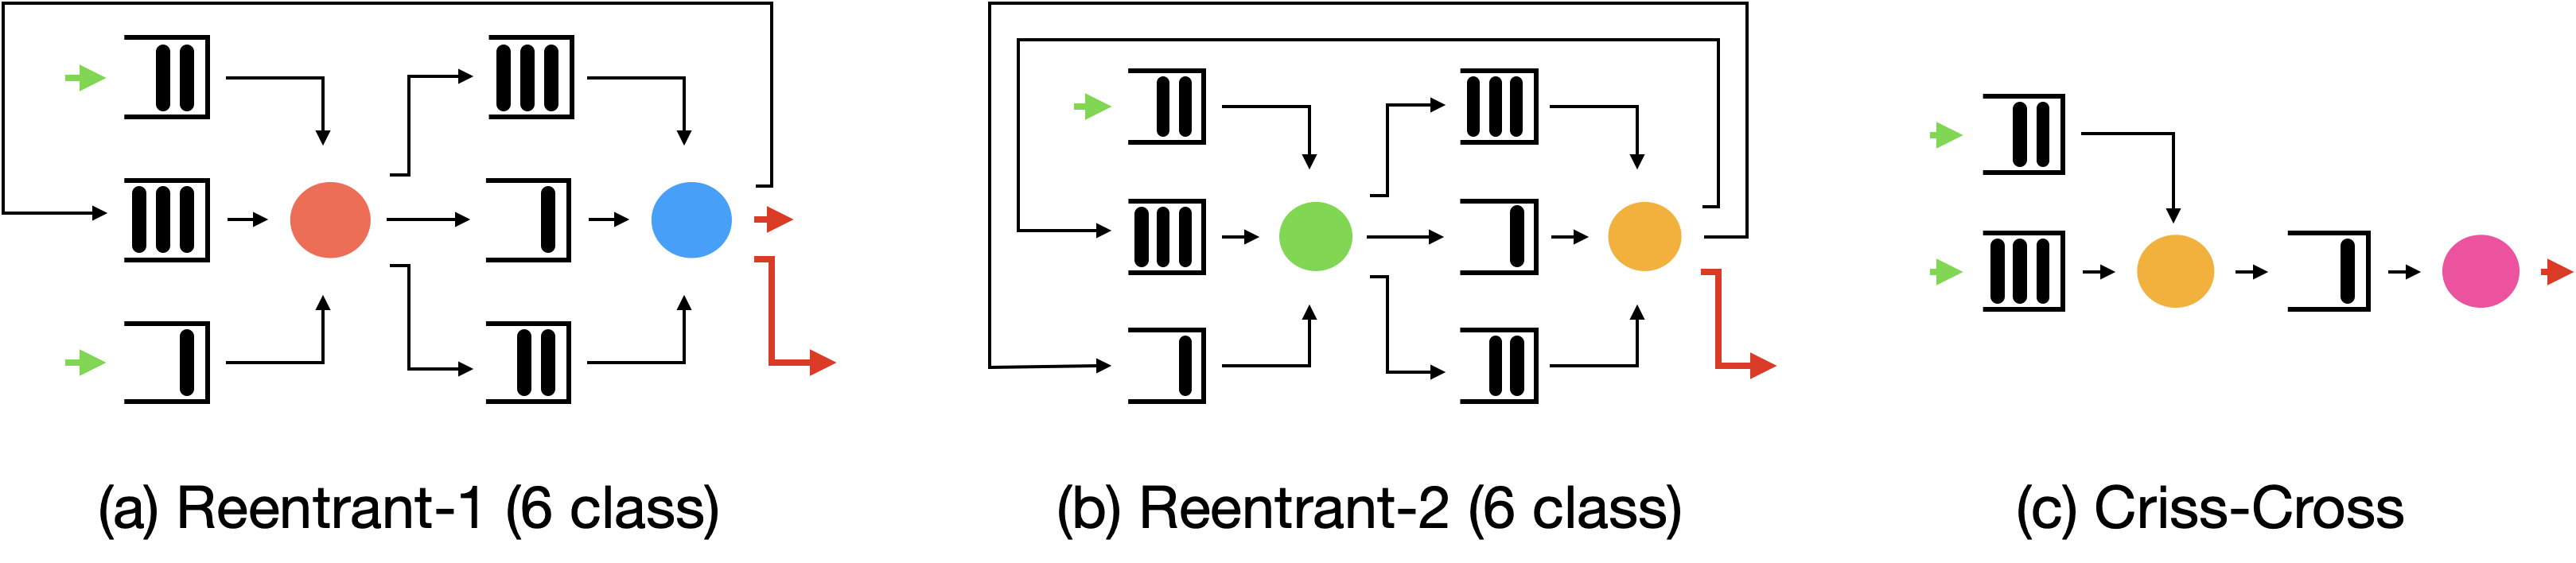
\includegraphics[height = 1.3in]{plot/results/queue_diagram.png} 
        \caption{Multi-class queuing networks. This figure displays the architectures for the networks considered in sections~\ref{section:gradient_eval} and~\ref{section:results}, and have appeared in previous works (see~\cite{dai2022queueing, bertsimas2014robust}). This displays the re-entrant networks with 6 job classes but we also consider networks with a larger number of job classes/queues. For both of these network architectures, the network with $n$ job classes has $n/3$ servers, and each job must be processed sequentially by all servers. Each server serves 3 job classes, and some of the jobs processed by the last server are fed back into the front of the re-entrant network.}

    \label{fig:networks} 
\end{figure}

% Beyond ensuring work-conservation, this constrains the behavior of the policy near the `boundaries' of the state space, i.e. where queue-lengths are zero, which would be otherwise difficult to learn from data using a smooth policy. To illustrate the usefulness of this property, recall the multi-class single-server queue in Example~\ref{example:multiclass}. It is well known that the $c\mu$-rule $\pi^{*}(x) = \arg \max_{j} h_{j} \mu_{j}1 \{x_{j} > 0 \}$ is an optimal scheduling policy. Since there is only 1 server, we omit the indexing for servers. 

% Our basic point is that because the boundary term $1 \{x_{j} > 0 \}$ appears in the work-conserving softmax, we can easily approximate this policy with a `simple' $\nu(x)$ that is \emph{static} across $x$. 


% \begin{proposition}
%     In a multi-class, single-server queue with with $n$ queues. Under the work-conserving softmax,
%     a static score $\nu_{\theta}(x)_{j} = \beta \theta_{j}$ for $\theta \in \R^{n}$, $\beta \in \R_{+}$ can approximate the optimal policy uniformly across the state-space, i.e. there exists $\theta \in \R^{n}$ such that, 
%     \[
%        \max_{j \in [n]}\max_{x \in \N^{n}} | \pi^{*}(x)_{j} - \pi_{\beta \theta}^{\mathsf{WC}}(x)_{j} | \leq \beta^{-1}  + \epsilon
%     \]
%     However, under the vanilla softmax $\pi_{\theta}(x)_{j} = \softmax(\nu_{\theta}(x))_{j}$,
%     any static policy incurs a constant approximation error. 
% \end{proposition}

% On the other hand, for the vanilla softmax to well-approximate the $c\mu$-rule it must learn this boundary behavior. This requires a `complex' $\nu(x)$ . We can formalize complexity as the Lipschitz constant of $\nu(x)$, where for any $g:\R^{n} \to \R$, the Lipschitz constant is defined as
% \[
% \mathsf{Lip}(g) \equiv \sup_{x,y\in \R^{n}} \frac{|g(x)-g(y)|}{\|x - y\|_{1}}
% \]
% where we use the $1$-norm for simplicity. The Lipschitz constant is a reasonable measure of complexity and can be used to bound other measures such as Rademacher complexity.  The static policy is simple in that its Lipschitz constant is zero.
% \begin{proposition}
%     In the multi-class, single-server queue, suppose that that $\pi_{\theta}(x) = \softmax(\nu_{\theta}(x))$ is a $\delta$ approximation to the $c\mu$-rule,
%     \[
%        \max_{j \in [n]}\max_{x \in \N^{n}} | \pi^{*}(x)_{j} - \pi_{\theta}(x)_{j} | \leq \delta
%     \]
%     Then it must be the case that
%     \[
%         \mathsf{Lip}\left( \nu(x)_{j} \right) \geq O\left( \log \left(\frac{1}{\delta} \right) \right), \quad \forall j = 1,...,n  
%     \]
% \end{proposition}
% % Intuitively, in order to learn the $c\mu$ policy, the vanilla softmax must approximate the boundary behavior
% % $1 \{x_{j} > 0 \}$, which can be difficult and requires the score $\nu(x)_{j}$ to be complex. On the other hand,
% % the work-conserving softmax has the boundary term $1 \{x_{j} > 0 \}$ already
% % embedded in the policy and doesn't need to learn it. As a result, it is able to approximate the optimal policy
% % with a simple static 
% One can still well-approximate this behavior using the vanilla-softmax, e.g. by setting $\nu(x)=\beta \cdot h_{j}\mu_{j} \min \{x,1\}$ and letting $\beta \to \infty$, but this is still more complex than a static $\nu(x)$. By embedding this boundary behavior into the whether the difficulties in applying deep reinforcement learning are due to
% the fundamental hardness of the problem or due to the difficulty of learning this boundary behavior
% using data.

% Despite the simplicity of this approach and the dramatic benefits it brings, this has so far not been
% proposed in previous approaches for applying RL in queuing. Rather, these approaches have mainly focused
% on constraining the policy when the queue-lengths are large. Surprisingly, the success of this simple modification
% suggests that it is more important to constrain the behavior near the boundary.